\documentclass[a4paper, 11pt]{scrartcl}

\usepackage[utf8]{inputenc}
\usepackage[ngerman]{babel}

\usepackage{mathptmx}
\renewcommand{\familydefault}{\sfdefault}
\usepackage[left=2.2cm, right=2.2cm, top=2.2cm, bottom=1.8cm]{geometry}
\usepackage[onehalfspacing]{setspace}

% \usepackage{hyperref}
\usepackage{amsmath}
\usepackage{amssymb}
\usepackage{graphicx}
\usepackage{xcolor}
\usepackage{floatflt,epsfig}
\usepackage{scrlayer-scrpage}
\usepackage{hyperref}
\usepackage{float}
\usepackage{sectsty}

\usepackage{xcolor}
\usepackage{floatflt,epsfig}
% \usepackage[fleqn]{amsmath}
\usepackage{listings}
\usepackage{color}
%\usepackage{minted}

\definecolor{dkgreen}{rgb}{0,0.6,0}
\definecolor{gray}{rgb}{0.5,0.5,0.5}
\definecolor{mauve}{rgb}{0.58,0,0.82}

\lstset{
    language=bash,
    aboveskip=3mm,
    belowskip=3mm,
    showstringspaces=false,
    columns=flexible,
    basicstyle={\small\ttfamily},
    numbers=none,
    numberstyle=\tiny\color{gray},
    keywordstyle=\color{mauve},
    commentstyle=\color{dkgreen},
    stringstyle=\color{blue},
    breaklines=true,
    breakatwhitespace=true,
    tabsize=3,
    morekeywords={
        sudo, apt, git   
    }
}

\definecolor{BBS}{RGB}{0,169,164}

\sectionfont{\color{BBS}}
\subsectionfont{\color{BBS}}
\subsubsectionfont{\color{BBS}}

\begin{document}
% \begin{spacing}{1.3}
\thispagestyle{empty}
\ihead{
    \begin{footnotesize}
        Deployment einer Webapp
    \end{footnotesize}
}
\chead{
    \begin{footnotesize}
        Lernfeld 9: Netzwerke und Dienste bereitstellen
    \end{footnotesize}
}
\ohead{
    \begin{footnotesize}
        Gerrit Koppe
    \end{footnotesize}
}
\vspace{0.2\textheight}
\begin{center}
    \begin{figure}[H]
        \begin{minipage}{0.3\textwidth}
            
\includegraphics[scale=0.6]{Bilder/BBS}
        \end{minipage}
        \hspace{0.48\textwidth}
        \begin{minipage}{0.3\textwidth}
            
\includegraphics[scale=0.6]{Bilder/sievers.png}
        \end{minipage}
    \end{figure}
    \vspace{1cm}
    \begin{Huge}
        \textcolor{BBS}{\textbf{Dokumentation Deployment einer Rest API}}
    \end{Huge}
    \\
    \vspace{0.1\textheight}
    \begin{Large}
        Autor: Gerrit Koppe
    \end{Large}
    \\
    \vspace{0.5cm}
    \begin{Large}
        Ausbildungsberuf: Fachinformatiker für Anwendungsentwicklung
    \end{Large}
    \\
    \vspace{0.5cm}
    \begin{Large}
        Klasse: IFA12
    \end{Large}
    \\
    \vspace{0.5cm}
    \begin{Large}
        Lernfeld 9: Netzwerke und Dienste bereitstellen
    \end{Large}
    \\
    \vspace{0.5cm}
    \begin{Large}
        \today
    \end{Large}
\end{center}
\newpage
\thispagestyle{empty}
\tableofcontents
\newpage
\clearpage
\pagenumbering{arabic}
\section{Einleitung}
In dieser Dokumentation %TODO das hier muss noch fertig gemacht werden



\section{Vorbereitungen}




\section{Konfiguration der User}



\section{Konfiguration des Netzwerks}




\section{Konfiguration der Firewall}




\section{Installation Apache2}



\section{Inbetriebnahme Rest API}



\newpage
\section{Anlagen}
\subsection{Bilder}

\subsubsection{Konfiguration User}


\subsubsection{Konfiguration Netzwerk}




\subsubsection{Konfiguration Firewall}
\begin{figure}[H]
    \begin{center}
        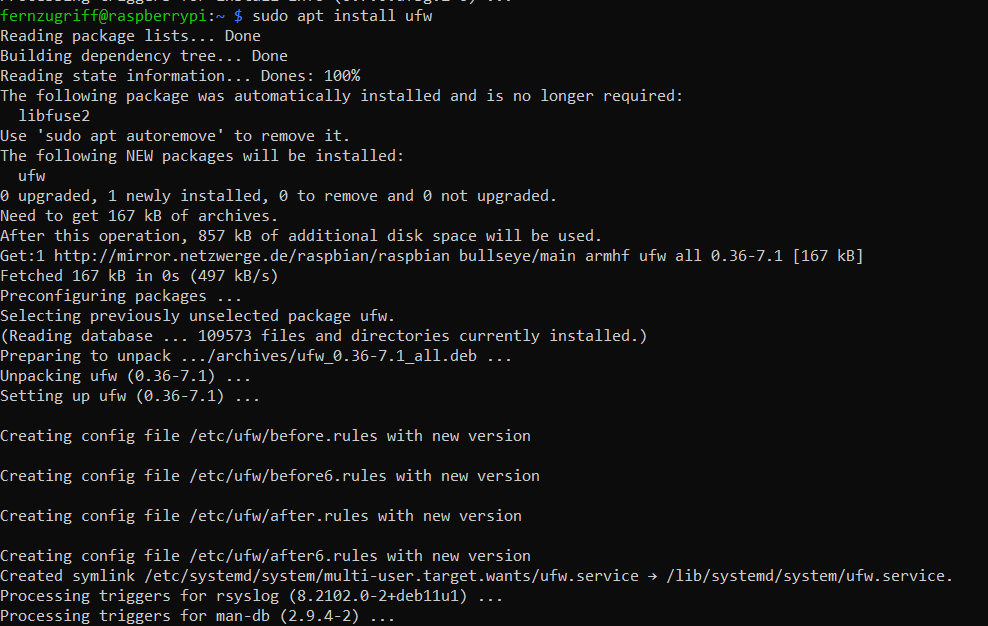
\includegraphics[scale=0.7]{Bilder/install_firewall.png}
        \caption{Installation der UFW Firewall}\label{pic:install_firewall}
    \end{center}
\end{figure}

\begin{figure}[H]
    \begin{center}
        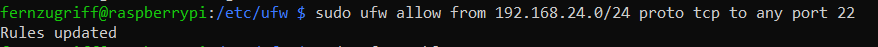
\includegraphics[scale=0.7]{Bilder/allow_ssh_from_network.png}
        \caption{SSH Port für gleiches Netzwerk öffnen}\label{pic:ssh_port_allow}
    \end{center}
\end{figure}

\begin{figure}[H]
    \begin{center}
        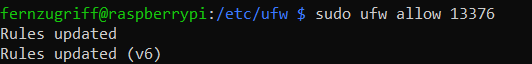
\includegraphics[scale=0.7]{Bilder/ufw_allow_api.png}
        \caption{Port der API für alle Netzwerke freischalten}\label{pic:api_port_allow}
    \end{center}
\end{figure}

\begin{figure}[H]
    \begin{center}
        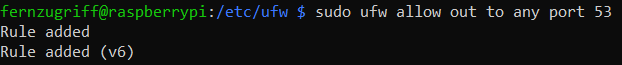
\includegraphics[scale=0.7]{Bilder/ufw_allow_out_dns.png}
        \caption{Ausgehende DNS Anfragen erlauben}\label{pic:dns_allow_out}
    \end{center}
\end{figure}

\begin{figure}[H]
    \begin{center}
        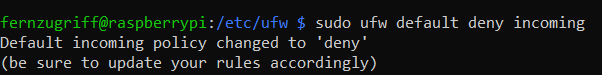
\includegraphics[scale=0.7]{Bilder/ufw_deny_all_incoming.png}
        \caption{Alle eingehenden Pakete ohne Regel verbieten}\label{pic:firewall_deny_default}
    \end{center}
\end{figure}

\begin{figure}[H]
    \begin{center}
        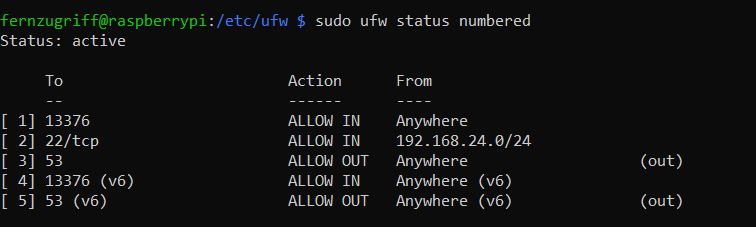
\includegraphics[scale=0.7]{Bilder/ufw_status_all_rules.png}
        \caption{Übersicht aller angelegten Regeln}\label{pic:firewall_status}
    \end{center}
\end{figure}





\subsection{Quellen}
\begin{small}

\end{small}
\end{document}